\section{Implementation}

For the project, all the focus was made to achieve the next core requirements:
\begin{itemize}
    \item Achieve both a simulated and real deployment of the required nodes.
    \item Real and simulated sensors are used, finally actuators such a virtual speaker are simulated.
    \item Intelligence distributed both in the nodes and in the edge platform.
    \item Possibility to command the network to stop the sensing.
    \item Fusion of information in the Edge Platform. This must result on some decisions and visual representations of the system's global state.
    \item A solution must be implemented to support future knowledge extraction in the system.
\end{itemize}

An important factor for the implementation of this project was the limited access to a \acrshort{lorawan} gateway. To solve the communication part, MQTT was used, as the edge 
platform supports this communication protocol by default.

\subsection{Sensing nodes}

In this project, two distinct nodes were developed, each with its specific characteristics. On one hand, we have a node equipped with sensors for presence detection, 
periodic measurements of temperature, humidity, wind, smoke, and flame detection via infrared sensors, located at the perimeter of the field. On the other hand, a 
simpler node equipped with an accelerometer is placed on the fence delimiting the crop field to detect potential unauthorized crossings.

\subsubsection*{Pir Node}


These nodes are positioned along the perimeter of the field. These PIR Nodes are built using the \texttt{PI PICO-W} board\cite{picowdatasheet}. This board is used 
for it's utility in fast deployment and possibility for Wi-Fi and \acrfullr{ble}. This node has the capability of sending the information related to:
\begin{itemize}
    \item 2 real PIR Sensors, one for each side. The sensor used for this is the \texttt{HC-SR501}\cite{MANUALDELUSUARIOSENSORDEMOVIMIENTOPIRHCSR501}. This sensor was selected for it's adjustability and low power consumption.
    \item 2 Infrared Sensors to help detect fires near the sensor.
    \item An MQ-2 smoke sensor\cite{mq2} to analyze the presence of alarming particles in the air.
    \item A temperature and humidity sensor from \texttt{Adafruit}\cite{DHT11basictemperaturehumidity}.
    \item A wind speed sensor. In this project this sensor is simulated due to the time constraints, but the support for the data it's included.
    \item A GPS Module is also simulated.
\end{itemize}

Finally, to represent the actuation of the network over the system. Two LEDs are used:
\begin{itemize}
    \item Red led to represent the status of the system (Sending data or not).
    \item Yellow led to represent the activation of the speaker of the node to scare wild animals.
\end{itemize}

The node is presented in the \autoref{fig:PIRFisico}.

\begin{figure}[H]
    \centering
    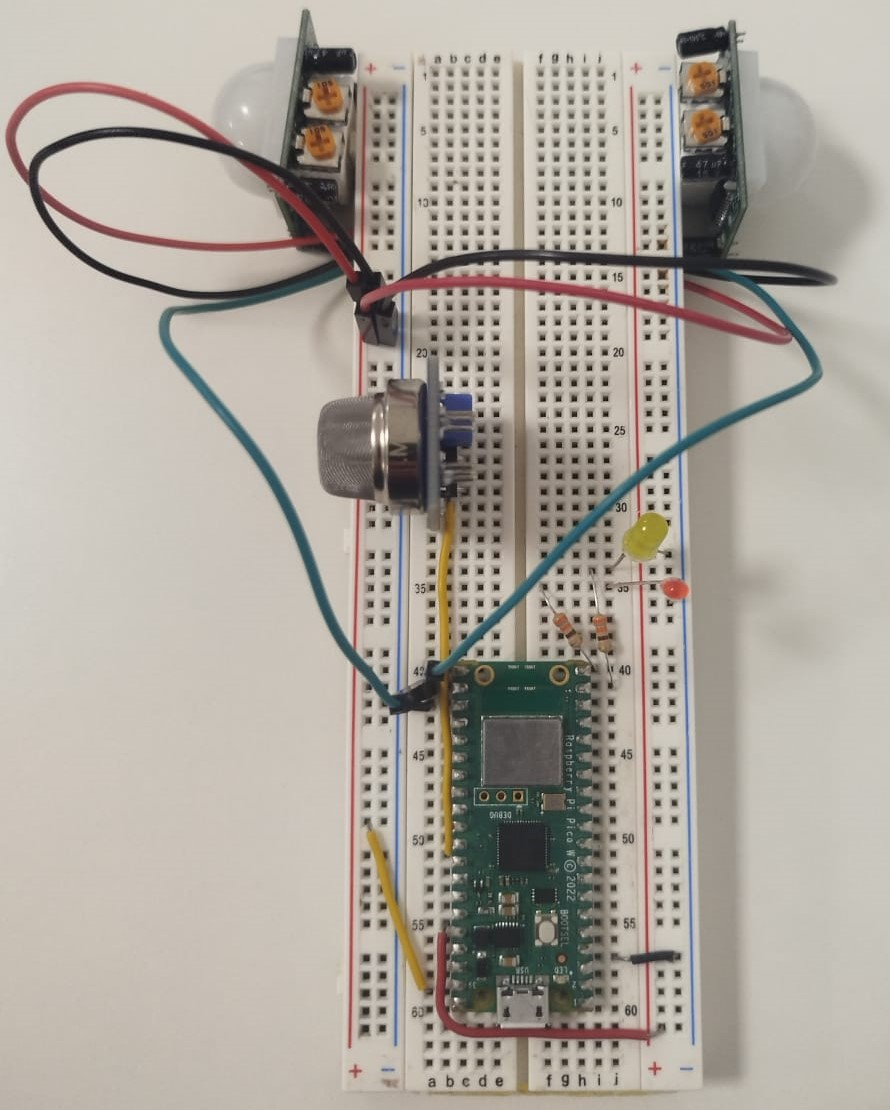
\includegraphics[width=0.85\textwidth,angle=-90]{./images/8/PIRNode.jpg}
    \caption{Final PIR Node}
    \label{fig:PIRFisico}
\end{figure}

\clearpage
\subsubsection*{Fence Node}

These nodes are positioned along the perimeter of the field, in the positions between the PIR nodes. The Fence Node contains an accelerometer that will sense 
any movements in the fence and send information with interruptions generated by the accelerometer. This node uses as the \acrshort{mcu} an ESP32\cite{esp32wroom32_datasheet_en}. The accelerometer is an \texttt{MPU-6050}\cite{MPU6000Datasheet1}. The node is presented in the next figure:

\begin{figure}[H]
    \centering
    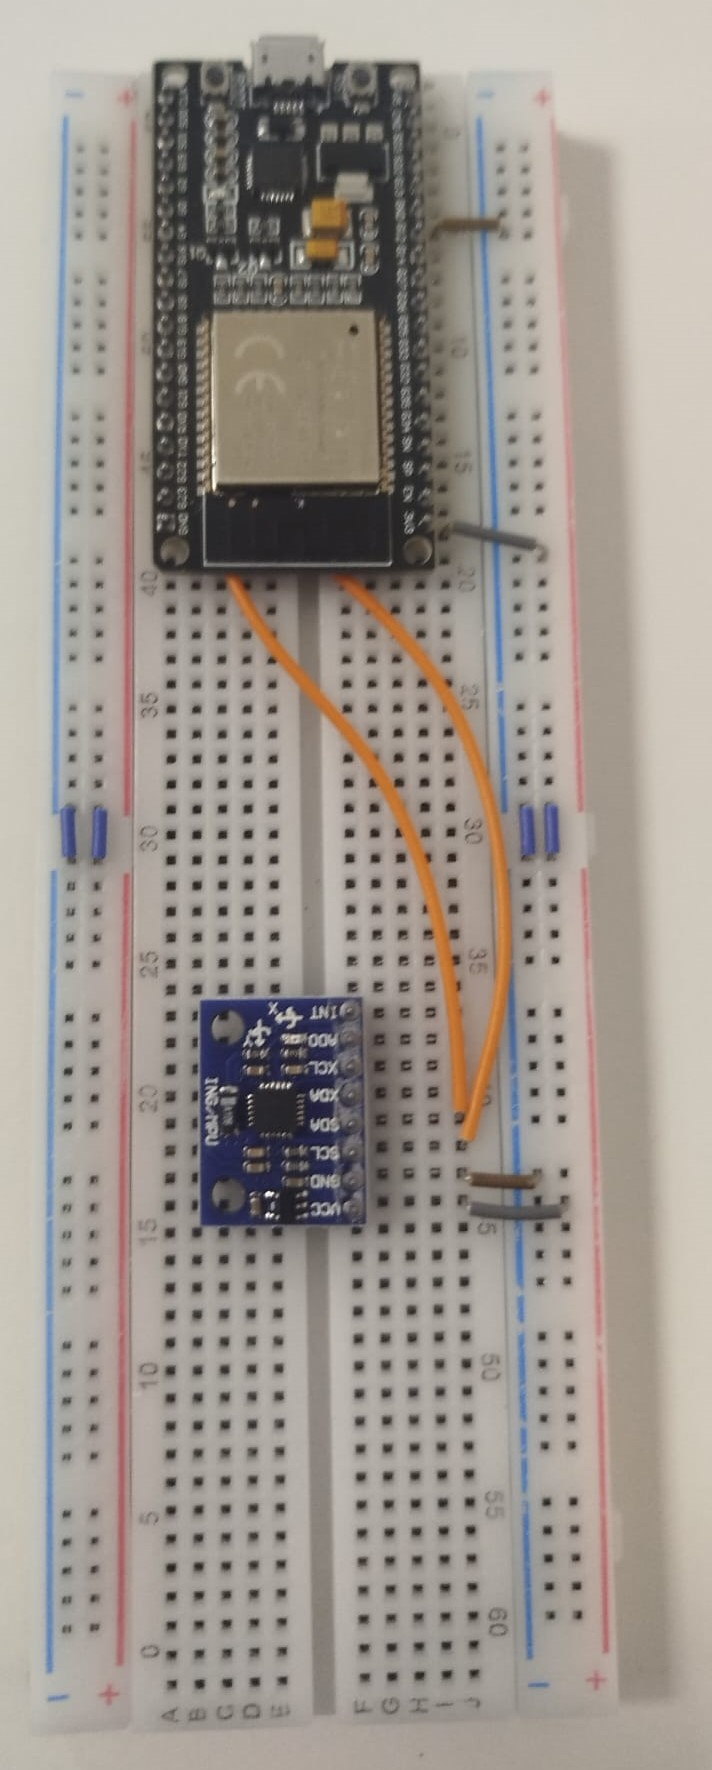
\includegraphics[width=0.4\textwidth,angle=-90]{./images/8/FENCENode.jpg}
    \caption{Final Fence Node}
    \label{fig:FENCEFisico}
\end{figure}

\subsection{Edge Computing: ThingsBoard Platform}

\subsubsection*{Devices and Assets Profiles}

To manage the information from all the sensors, actuators, and elements involved in this system within the Thingsboard platform, we utilize virtual representations of 
these components through Devices and Assets. Devices represent each node virtually, while assets represent the corresponding physical elements. For our use cases, we 
distinguish between the two types of nodes, each with its own device profile, and define one asset type as listed below:
\begin{itemize}
    \item PIR Node Profile.
    \item Fence Node Profile.
    \item Presence Asset Profile. This Asset Profile indicates real-time presence detection for each fence section. It differentiates between a presence detected on 
    a single side, multiple detections, or a possible unauthorized crossing.
\end{itemize}

For this project, and considering the specified constraints, we deployed a total of 8 devices to cover the perimeter of the crop field—4 devices for each defined Device 
Profile. Additionally, we defined 4 assets using the Presence Asset Profile type, representing the presence detected by each fence segment. \autoref{fig:NodesSchematic} provides a schematic 
representation of the nodes and assets placement.
\begin{figure}[H]
    \centering
    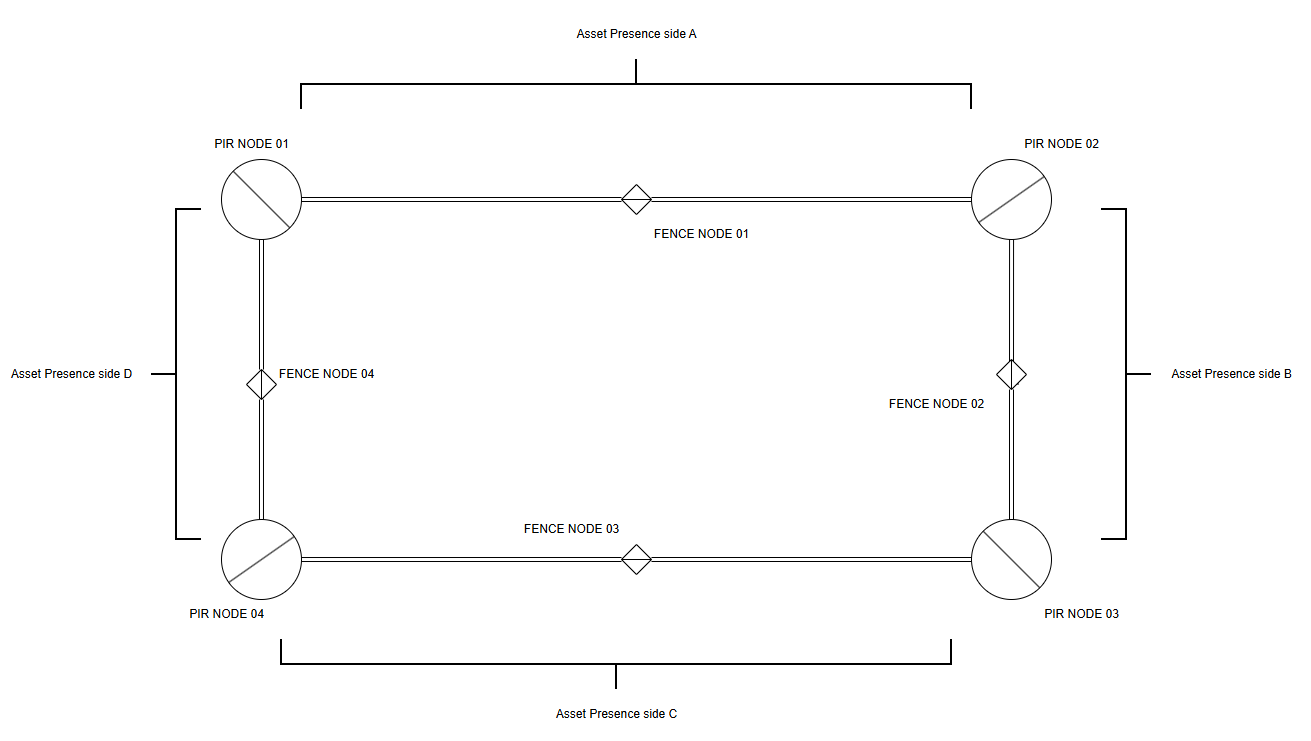
\includegraphics[width=1\textwidth]{./images/8/NodesSchematic.PNG}
    \caption{Node Schema}
    \label{fig:NodesSchematic}
\end{figure}

To detect presence or crossings effectively, the PIR Node Devices are configured with relationships to two neighboring PIR Nodes and two defined assets. These relationships 
are as follows (the terms left and right are oriented outward from the crop field):
\begin{itemize}
    \item (\texttt{leftneighbour}): Links a PIR Node to the PIR Node located to its left.
    \item (\texttt{rightneighbour}): Links a PIR Node to the PIR Node located to its right.
    \item (\texttt{leftpresence}): Links a PIR Node to the Presence Asset on its left side.
    \item (\texttt{rightpresence}): Links a PIR Node to the Presence Asset on its right side.
    \item (\texttt{features}): Links a Fence Node to the Presence Asset associated with its section.
\end{itemize}
By leveraging these relationships, the system can monitor detected presences, determine which side of the field they occur on, and generate appropriate alarms accordingly. 
Therefore, the relationships for each node, based on the previous diagram, would be as indicated below:



\subsubsection*{Rule Chains}
In this project, two distinct nodes were developed, each with its specific characteristics. On one hand, we have the PIR node and on the other hand, the fence node. 
Each device profile is assigned a specific Rule Chain to analyze the data received from the node devices and trigger the corresponding alarms.


\subsubsection*{PIR Node Analyzer}
The alarms generated by this Rule Chain include:
\begin{itemize}
    \item Fire Detected.
    \item Fire Hazard.
    \item Presence Detected.
\end{itemize}

The Rule Chain first validates that all required fields are present in the incoming message. If the message format is incorrect or incomplete, an alarm is triggered 
to indicate that the incoming message cannot be processed. Once the message format is validated, the data is parsed for easier subsequent processing, producing a JSON
structure similar to the one shown in \autoref{fig:parsedJson}.

\begin{figure}[H]
    \centering
    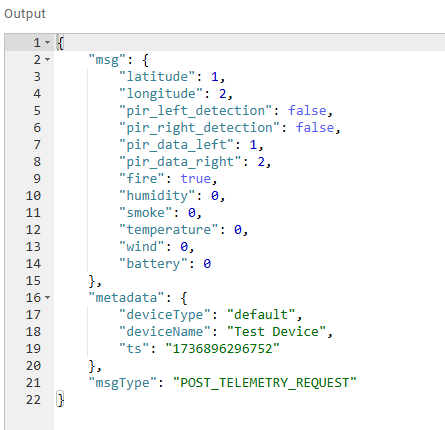
\includegraphics[width=0.6\textwidth]{./images/8/jsonParsed.PNG}
    \caption{Parsed JSON for Rule Chain Processing}
    \label{fig:parsedJson}
\end{figure}

Fire detection relies on the value in the \texttt{fire} field. In the Check Fire node of the Rule Chain, if the \texttt{fire} field returns \texttt{true}, a critical alarm for "Fire Detected"
is triggered. If the value is \texttt{false}, the alarm is deactivated.

The "Fire Hazard" alarm is activated by evaluating the parameters for temperature, humidity, wind speed, and smoke levels. According to some studies\cite{norma303030tres}, the conditions 
for a fire hazard include:
\begin{itemize}
    \item Temperature above $30$°$C$.
    \item Relative humidity below $30\%$.
    \item Wind speeds exceeding $30 km/h$.
\end{itemize}

Additionally, a smoke concentration exceeding 200 \acrfullr{ppm} triggers the alarm. If none of these conditions are met, the alarm is deactivated.

For presence detection, four PIR nodes are placed at each vertex of the square representing the crop field. The field is divided into four zones corresponding to each side 
of the polygon. The presence detection algorithm works as follows:
\begin{itemize}
    \item If a presence is detected by a PIR sensor (indicated by 'pir\_XX\_detection', where XX can be 'left' or 'right'):
    \begin{itemize}
        \item The status of the opposite side’s neighboring node is checked.
        \item If the neighboring node also reports presence (\texttt{true}) within a timespan of 10 seconds, the "Presence Detected" alarm is triggered, and a speaker is activated.
        \item If no presence is detected on the opposite side, a lower-priority alarm is triggered, indicating presence on one side of the fence.
    \end{itemize}
    \item If no presence is detected on the initial node, all related presence alarms are deactivated. 
\end{itemize}

The pseudocode for this logic is as follows:
\lstinputlisting[caption={Presence Algorithm}, label={lst:presence}]{code/presence.c}

To implement this algorithm, relationships between the various nodes and assets were defined. Accessing values from neighboring nodes was achieved through the Change
Originator node in Thingsboard, which specifies the target node using the predefined relationships. Similarly, the originator change process is used to update related 
asset values. The full flow of the Rule Chain is illustrated in \autoref{fig:PirNodeAnalyzer}.

\begin{figure}[H]
    \centering
    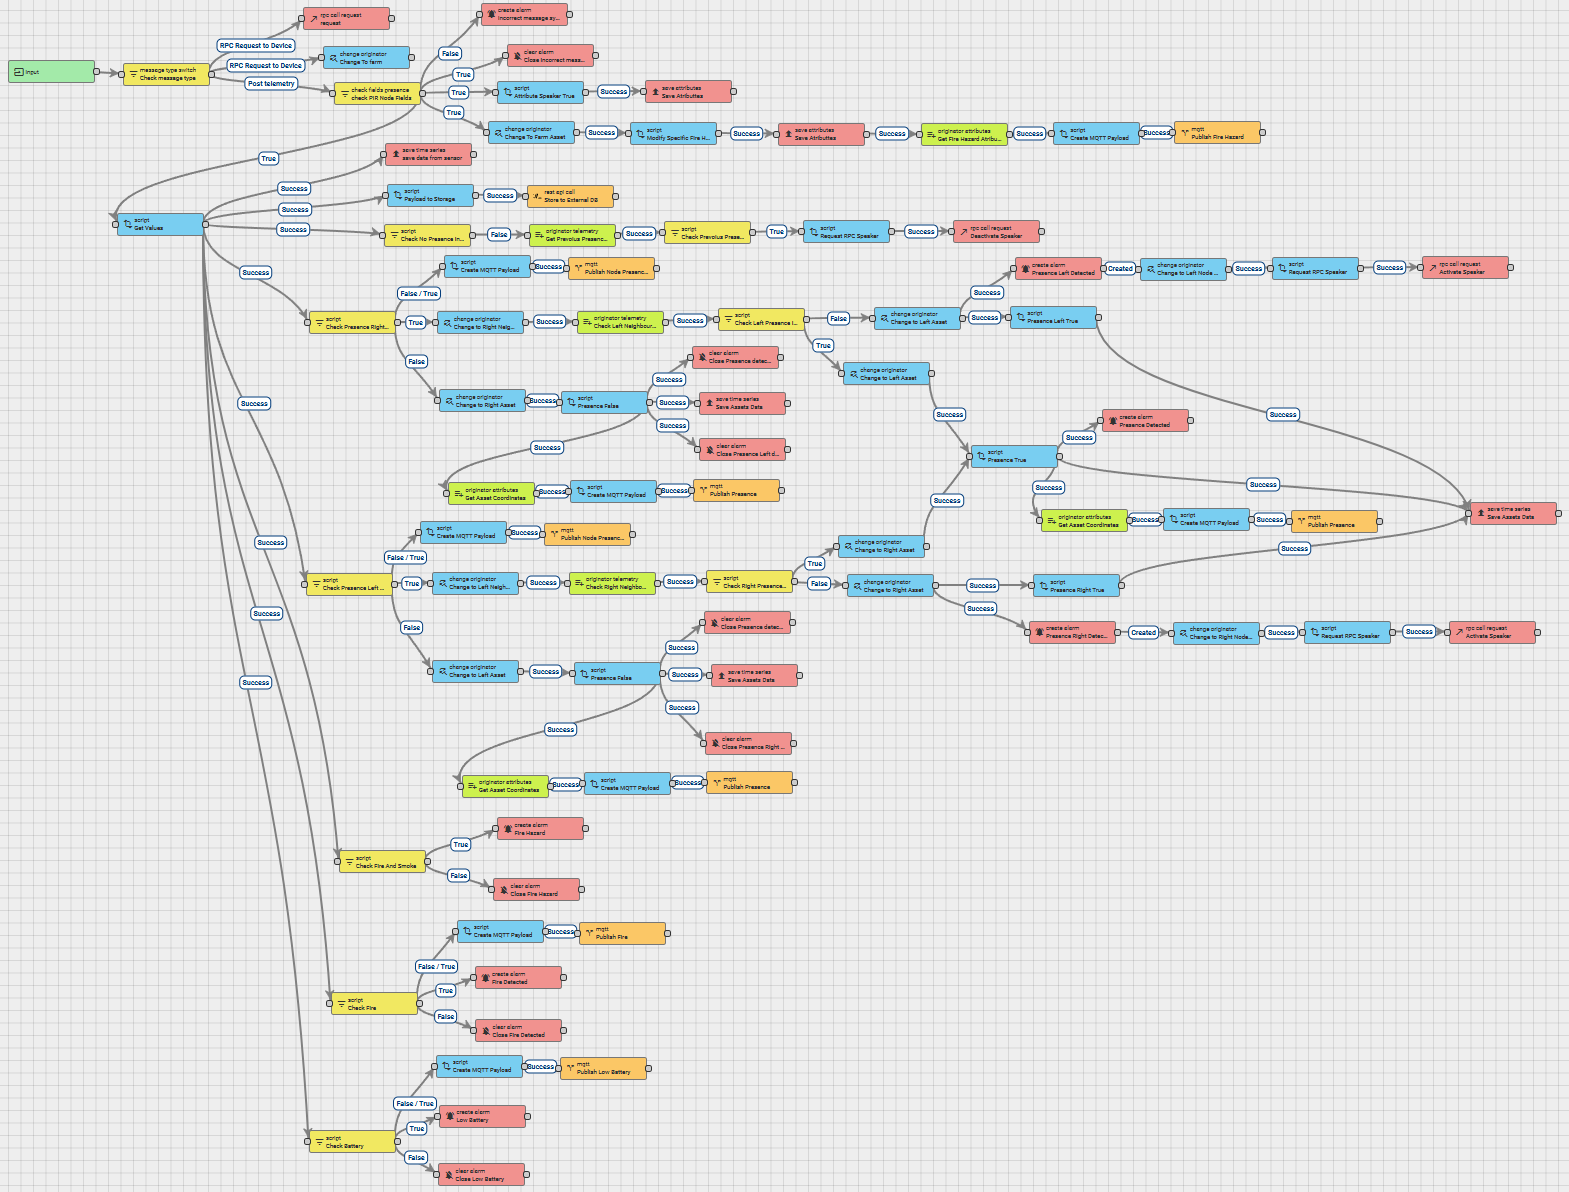
\includegraphics[width=1.4\textwidth,angle=90]{./images/8/PirNodeAnalyzer.PNG}
    \caption{PIR Node Analyzer Rule Chain FLow}
    \label{fig:PirNodeAnalyzer}
\end{figure}

\subsubsection*{Fence Node Analyzer}
This Rule Chain is designed to process messages from nodes placed on the fence to detect movements and generate alarms accordingly.  
Similar to the previous Rule Chain, it first validates that all required fields are present in the incoming message. However, since this node is simpler, the Rule 
Chain specifically generates the "Fence Trespassed" alarm based on the value of the 'acceleration\_interruption' field. The flow of this process is illustrated in \autoref{fig:FenceNodeAnalyzer}.

\begin{figure}[H]
    \centering
    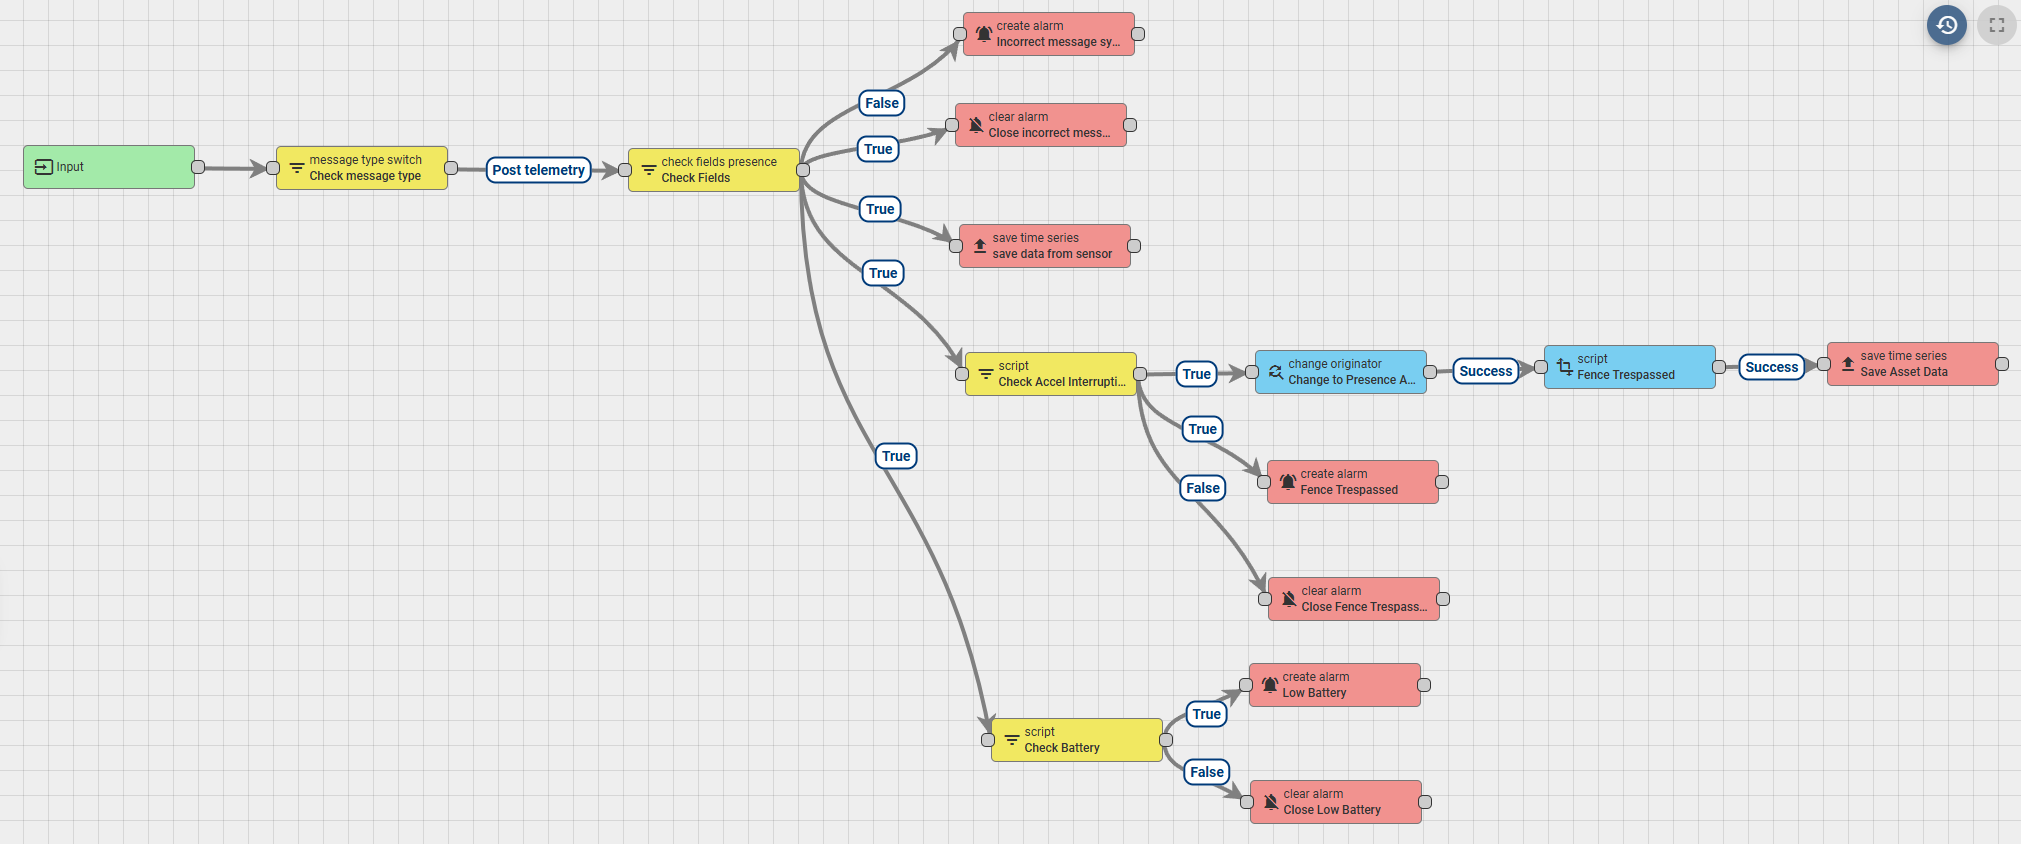
\includegraphics[width=1\textwidth]{./images/8/FenceNodeAnalyzer.PNG}
    \caption{Fence Node Analyzer Rule Chain FLow}
    \label{fig:FenceNodeAnalyzer}
\end{figure}

\subsubsection*{Dashboard}

To represent all the information generated during the processing of the aggregated data. The dashboard 
functionality from ThingsBoard was used. To implement the dashboard utilities like aliases and dashboard 
states were used.

The dashboard defined 2 views implemented with states:
\begin{itemize}
    \item The map dashboard, that shows the status of the farm perimeter and the different PIR nodes. This map can also change colors in reaction 
    to some events, like presence detection or fire detection. This also affects the markers of the nodes. Finally, the nodes can be clicked to obtain 
    a summarized view of the state of the node and the latest telemetry. This view is presented in \autoref{fig:MapThingsboard}.
    \begin{figure}[H]
        \centering
        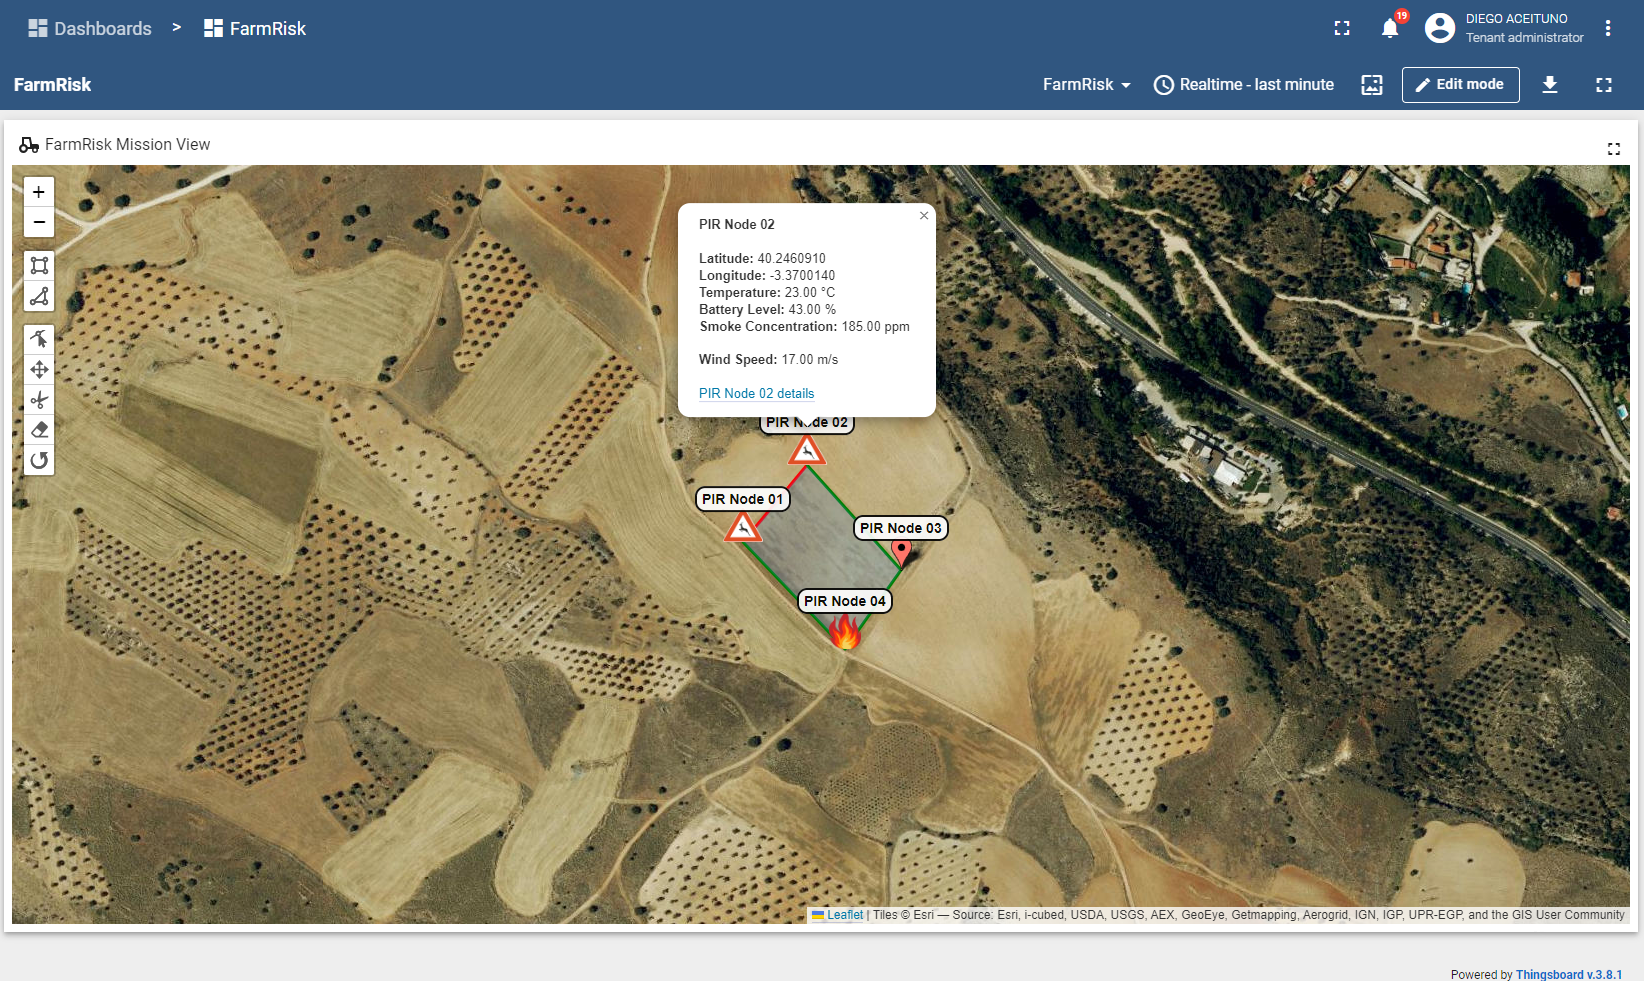
\includegraphics[width=1\textwidth]{./images/8/MapDashboard.png}
        \caption{Map dashboard implemented in Thingsboard}
        \label{fig:MapThingsboard}
    \end{figure}
    \item When any tooltip's "further details" is clicked, the dashboard changes to the sensor view of the sensor clicked. This dashboard 
    shows time series data and further details about the state of the sensor. This view is presented in \autoref{fig:NodeThingsboard}. 
    \begin{figure}[H]
        \centering
        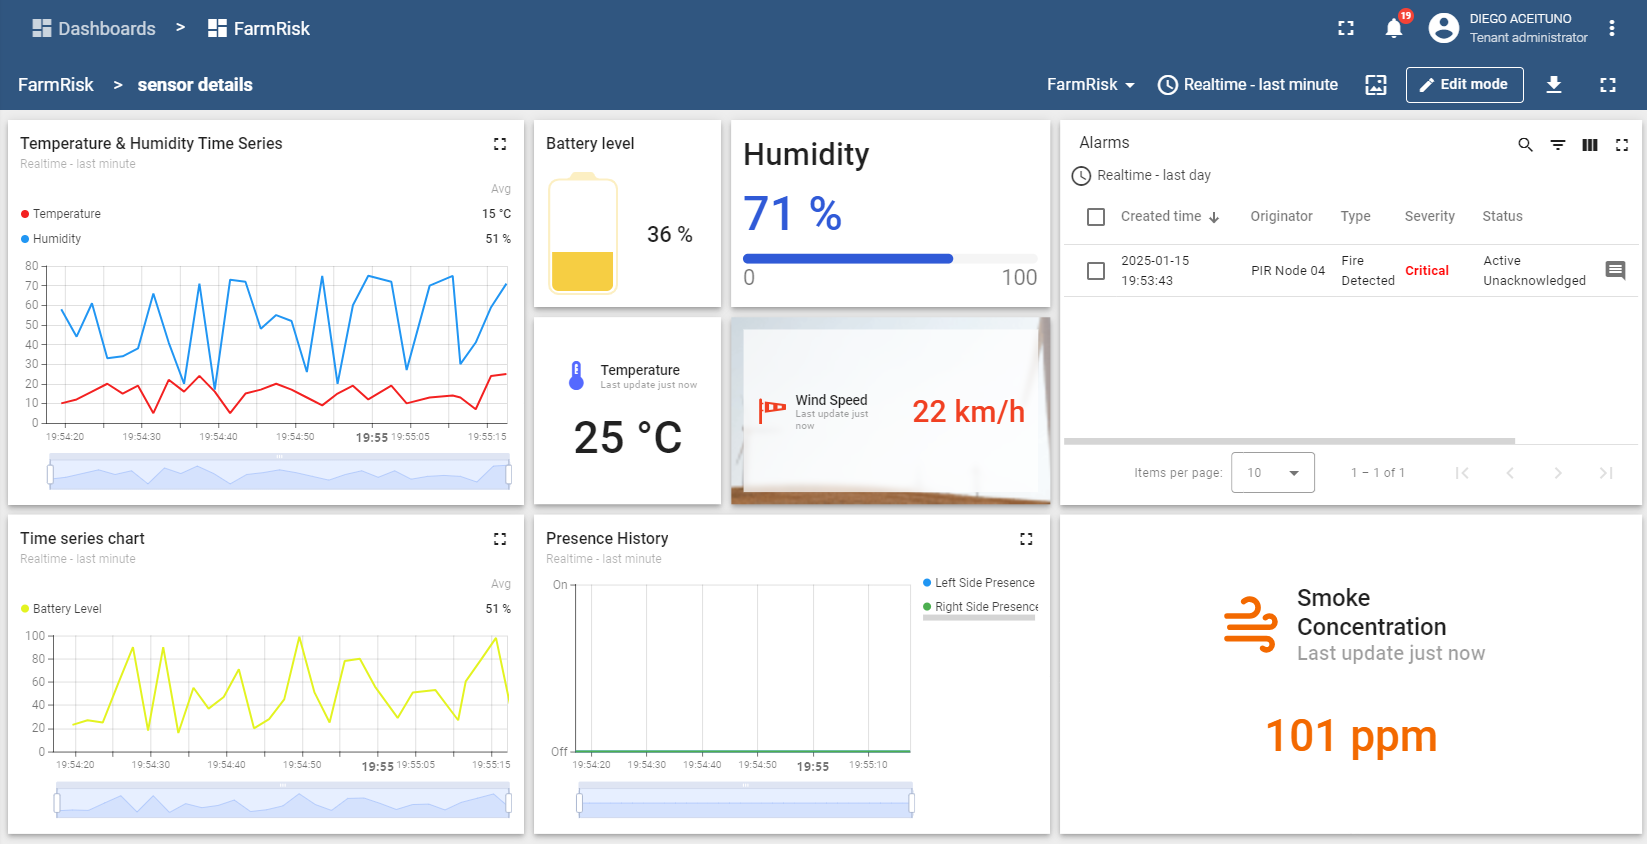
\includegraphics[width=1\textwidth]{./images/8/NodeDashboard.png}
        \caption{Node dashboard implemented in Thingsboard}
        \label{fig:NodeThingsboard}
    \end{figure}
\end{itemize}
